\documentclass[11pt, a4paper]{article}
\usepackage[utf8]{inputenc}
\usepackage[T1]{fontenc}
\usepackage{amsmath, amssymb, amsthm, mathtools}
\usepackage[margin=0.85in]{geometry}
\usepackage{hyperref}
\hypersetup{colorlinks=true, linkcolor=blue!70!black, urlcolor=teal,
    pdftitle={HSMA: Holographic Spin-Manifold Architecture v4.0 — The Complete Specification},
    pdfauthor={Sk Sarin Arfin}}
\usepackage{listings}
\usepackage{xcolor}
\usepackage{booktabs}
\usepackage{longtable}
\usepackage{array}
\usepackage{titlesec}
\usepackage{enumitem}
\usepackage{graphicx}
\usepackage{tikz}
\usetikzlibrary{arrows.meta, positioning, shapes.geometric, decorations.pathreplacing,
                calc, shadows.blur, backgrounds, fit}
\usepackage{algorithm}
\usepackage{algpseudocode}
\usepackage{tcolorbox}
\tcbuselibrary{skins, breakable}

% ═══════════════ COLOR PALETTE ═══════════════════════════════════
\definecolor{hsmaBlue}{RGB}{0,70,150}
\definecolor{hsmaTeal}{RGB}{0,130,130}
\definecolor{hsmaGreen}{RGB}{0,140,60}
\definecolor{hsmaRed}{RGB}{180,30,30}
\definecolor{hsmaGold}{RGB}{184,134,11}
\definecolor{hsmaPurple}{RGB}{100,40,160}
\definecolor{hsmaDark}{RGB}{15,25,45}
\definecolor{hsmaOrange}{RGB}{230,120,0}
\definecolor{codebg}{RGB}{243,246,251}
\definecolor{theorembg}{RGB}{235,245,255}
\definecolor{defnbg}{RGB}{255,248,235}
\definecolor{receiptbg}{RGB}{235,252,235}
\definecolor{warnbg}{RGB}{255,240,240}
\definecolor{infobg}{RGB}{240,240,255}
\definecolor{tablehdr}{RGB}{0,70,150}
\definecolor{rowalt}{RGB}{240,245,252}

\lstdefinestyle{cppstyle}{
    language=C++, backgroundcolor=\color{codebg},
    basicstyle=\ttfamily\footnotesize,
    keywordstyle=\color{hsmaPurple}\bfseries,
    commentstyle=\color{hsmaGreen}\itshape,
    stringstyle=\color{hsmaRed},
    numbers=left, numberstyle=\tiny\color{codegray},
    frame=single, rulecolor=\color{hsmaBlue!40},
    breaklines=true, tabsize=2,
    showstringspaces=false,
    morekeywords={constexpr, noexcept, uint8_t, uint32_t, uint64_t, size_t}
}
\lstdefinestyle{bashstyle}{
    language=bash, backgroundcolor=\color{hsmaDark},
    basicstyle=\ttfamily\footnotesize\color{hsmaGreen},
    keywordstyle=\color{hsmaGold}\bfseries,
    numbers=none, frame=none
}

\lstset{style=cppstyle}

% ═══════════════ SECTION FORMATTING ══════════════════════════════
\titleformat{\part}
    {\centering\Huge\bfseries\color{hsmaDark}}{\partname~\thepart}{1em}{}
    [{\color{hsmaBlue}\titlerule[2pt]}]
\titleformat{\section}
    {\LARGE\bfseries\color{hsmaBlue}}{\thesection}{1em}{}
    [{\color{hsmaBlue!60}\titlerule[1.2pt]}]
\titleformat{\subsection}
    {\Large\bfseries\color{hsmaTeal}}{\thesubsection}{1em}{}
\titleformat{\subsubsection}
    {\large\bfseries\color{hsmaDark}}{\thesubsubsection}{1em}{}
\titlespacing{\section}{0pt}{2.5em}{1.2em}
\titlespacing{\subsection}{0pt}{1.8em}{0.8em}

% ═══════════════ THEOREM ENVIRONMENTS ════════════════════════════
\theoremstyle{plain}
\newtheorem{theorem}{Theorem}
\newtheorem{lemma}[theorem]{Lemma}
\newtheorem{corollary}[theorem]{Corollary}
\newtheorem{proposition}[theorem]{Proposition}
\theoremstyle{definition}
\newtheorem{definition}{Definition}
\newtheorem{invariant}{Invariant}
\newtheorem{axiom}{Axiom}
\theoremstyle{remark}
\newtheorem{remark}{Remark}
\newtheorem{conjecture}{Conjecture}
\newtheorem{observation}{Observation}

% ═══════════════ TCOLORBOX ENVIRONMENTS ══════════════════════════
\newtcolorbox{theorembox}[1]{
    enhanced, breakable,
    colback=theorembg, colframe=hsmaBlue,
    fonttitle=\large\bfseries,
    title={#1},
    boxrule=1.2pt, arc=3mm,
    left=6pt, right=6pt, top=6pt, bottom=6pt,
    drop fuzzy shadow=hsmaBlue!30
}
\newtcolorbox{defnbox}[1]{
    enhanced, breakable,
    colback=defnbg, colframe=hsmaGold,
    fonttitle=\large\bfseries,
    title={#1},
    boxrule=1.2pt, arc=3mm,
    left=6pt, right=6pt, top=6pt, bottom=6pt,
    drop fuzzy shadow=hsmaGold!30
}
\newtcolorbox{receiptbox}[1]{
    enhanced, breakable,
    colback=receiptbg, colframe=hsmaGreen,
    fonttitle=\large\bfseries,
    title={#1},
    boxrule=1.2pt, arc=3mm,
    left=6pt, right=6pt, top=6pt, bottom=6pt,
    drop fuzzy shadow=hsmaGreen!30
}
\newtcolorbox{warnbox}[1]{
    enhanced, breakable,
    colback=warnbg, colframe=hsmaRed,
    fonttitle=\large\bfseries,
    title={#1},
    boxrule=1.2pt, arc=3mm,
    left=6pt, right=6pt, top=6pt, bottom=6pt,
    drop fuzzy shadow=hsmaRed!30
}
\newtcolorbox{infobox}[1]{
    enhanced, breakable,
    colback=infobg, colframe=hsmaPurple,
    fonttitle=\large\bfseries,
    title={#1},
    boxrule=1.2pt, arc=3mm,
    left=6pt, right=6pt, top=6pt, bottom=6pt,
    drop fuzzy shadow=hsmaPurple!30
}
\newtcolorbox{resultbox}[1]{
    enhanced, breakable,
    colback=hsmaGreen!5, colframe=hsmaGreen,
    fonttitle=\large\bfseries\color{white},
    colbacktitle=hsmaGreen,
    title={#1},
    boxrule=1.5pt, arc=3mm,
    left=8pt, right=8pt, top=8pt, bottom=8pt,
    drop fuzzy shadow=hsmaGreen!40
}

\newcommand{\hsma}{\textsc{hsma}}
\newcommand{\pie}{\pi_E}
\newcommand{\GATE}{\textsc{Gate Green}}
\newcommand{\cmark}{\textcolor{hsmaGreen}{\checkmark}}
\newcommand{\xmark}{\textcolor{hsmaRed}{$\times$}}
\newcommand{\fieldp}{\mathbb{F}_p}
\newcommand{\fieldq}{\mathbb{F}_q}

\begin{document}

% ══════════════════════════════════════════════════════════════════
% TITLE PAGE
% ══════════════════════════════════════════════════════════════════
\begin{titlepage}
\begin{tikzpicture}[remember picture, overlay]
    \fill[hsmaDark] (current page.north west) rectangle
        ([yshift=-6cm]current page.north east);
    \fill[hsmaBlue] ([yshift=-6cm]current page.north west) rectangle
        ([yshift=-6.15cm]current page.north east);
    \fill[hsmaTeal] ([yshift=-6.15cm]current page.north west) rectangle
        ([yshift=-6.3cm]current page.north east);
    \fill[hsmaGreen] ([yshift=-6.3cm]current page.north west) rectangle
        ([yshift=-6.45cm]current page.north east);
    \fill[hsmaGold] ([yshift=-6.45cm]current page.north west) rectangle
        ([yshift=-6.6cm]current page.north east);
    \fill[hsmaPurple] ([yshift=-6.6cm]current page.north west) rectangle
        ([yshift=-6.75cm]current page.north east);
    \fill[hsmaRed] ([yshift=-6.75cm]current page.north west) rectangle
        ([yshift=-6.9cm]current page.north east);
    \node[white] at ([yshift=-2cm]current page.north) {\fontsize{40}{48}\selectfont\bfseries HSMA};
    \node[hsmaTeal!80!white] at ([yshift=-3.2cm]current page.north)
        {\fontsize{22}{26}\selectfont\bfseries Holographic Spin-Manifold Architecture};
    \node[white!80] at ([yshift=-4.3cm]current page.north)
        {\large\itshape Not a Blockchain. Not a DAG.};
    \node[white!70] at ([yshift=-5.1cm]current page.north)
        {\normalsize A New Category of Protocol: Where Computation Becomes Consensus};
    \node[white!60] at ([yshift=-5.8cm]current page.north)
        {\small \texttt{github.com/sarinsk629-blip/hsma-core}};
\end{tikzpicture}

\vspace{4cm}

\begin{center}
{\LARGE\bfseries\color{hsmaDark} Technical Whitepaper}\\[0.3em]
{\Large\color{hsmaBlue} Version 4.0 --- The Complete Specification}\\[1.5em]
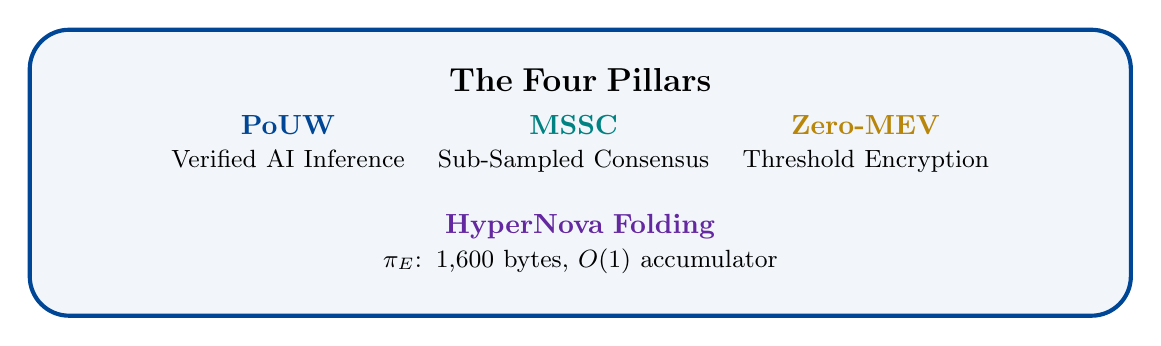
\begin{tikzpicture}
\node[rectangle, rounded corners=5mm, draw=hsmaBlue, line width=1.5pt,
      fill=hsmaBlue!5, inner sep=14pt, text width=13cm, align=center] {
    {\large\bfseries The Four Pillars}\\[6pt]
    \begin{tabular}{ccc}
    \textcolor{hsmaBlue}{\textbf{PoUW}} &
    \textcolor{hsmaTeal}{\textbf{MSSC}} &
    \textcolor{hsmaGold}{\textbf{Zero-MEV}} \\
    {\small Verified AI Inference} &
    {\small Sub-Sampled Consensus} &
    {\small Threshold Encryption} \\
    & \\
    \multicolumn{3}{c}{\textcolor{hsmaPurple}{\textbf{HyperNova Folding}}} \\
    \multicolumn{3}{c}{{\small $\pi_E$: 1{,}600 bytes, $O(1)$ accumulator}} \\
    \end{tabular}
};
\end{tikzpicture}

\vspace{1cm}

\begin{tabular}{ccc}
\textcolor{hsmaBlue}{\textbf{281}} & \textcolor{hsmaTeal}{\textbf{34}} & \textcolor{hsmaGreen}{\textbf{41}} \\
{\small Decisions} & {\small Gates Green} & {\small Golden Headers} \\[6pt]
\textcolor{hsmaGold}{\textbf{203}} & \textcolor{hsmaPurple}{\textbf{223}} & \textcolor{hsmaRed}{\textbf{1,600}} \\
{\small Laws} & {\small Defects Owned} & {\small Byte $\pi_E$} \\
\end{tabular}

\vfill
{\large Sk Sarin Arfin}\\[0.3em]
{\small Independent Research --- \texttt{sarinsk629@gmail.com}}\\[0.5em]
{\small September 2026}\\[1em]
{\small\itshape ``Impossible beats punishable.''}
\end{center}
\end{titlepage}

\begin{abstract}
We present \hsma{}, a protocol that does not fit the taxonomy of existing
decentralized systems. It is not a blockchain (there are no blocks). It
is not a DAG (there is no partial ordering). It is a \textbf{folding-based
state machine} whose consensus weight derives from \textit{verified AI
inference}, whose mempool is \textit{cryptographically unreadable before
ordering}, and whose entire epoch history compresses into a
\textit{1{,}600-byte recursive proof} verifiable without the witness in
118\,ms on phone-class hardware.

\hsma{} integrates four pillars into a single verified system:

\textbf{Verifiable AI Inference as Proof of Useful Work (PoUW).}
Consensus weight derives from GEMM matrix multiplications proven correct
via the sum-check protocol over the Pasta curve cycle. A $128^3$ matrix
multiplication comprising 2{,}097{,}152 multiply-accumulate operations
verifies in 1{,}422 bytes with $O(\log N)$ verifier work. The
aggregate-verify homomorphism achieves a measured 3.0$\times$ speedup at
 $N{=}3$, scaling to $\sim$224$\times$ at production committee size.

\textbf{Metastable Sub-Sampled Consensus (MSSC).} An Avalanche-family
protocol with weight-proportional sampling, beacon-gated stall breaking,
and a structural quorum impossibility guarantee ($\epsilon_{\text{quorum}}
= 0$ under $f < 0.20$ adversarial weight). The convergence property is
demonstrated at testnet scale: two nodes with conflicting initial
preferences resolve to one finalized state through the weight-weighted
sampling loop in 6 rounds. The wire-level convergence over real TCP with
BLS-signed votes is demonstrated.

\textbf{Zero-MEV Encrypted Mempool.} A Commit-then-Simulate ceremony
where transaction payloads are threshold-encrypted (224-member committee,
 $t{=}112$), the ordering is beacon-shuffled and committed \textit{before}
any decryption share exists, and the decrypted payloads feed the fold
pipeline. The complete ceremony is demonstrated end-to-end: 10 encrypted
envelopes $\to$ ordered $\to$ threshold-decrypted $\to$ folded $\to$  $\pi_E$ $\to$ PoUW weight. Front-running is structurally impossible:
nobody can front-run what nobody can read.

\textbf{Holographic State Folding.} HyperNova NIVC over the Pallas/Vesta
2-cycle folds heterogeneous state transitions into a 41-byte accumulator,
producing a recursive epoch proof $\pi_E$ (1{,}600 bytes, 2.2\% of the
73\,KB budget) verifiable without the witness.

All four pillars are connected: encrypted envelopes enter the mempool,
the ordering ceremony commits the sequence, the threshold decrypt unlocks
the payloads, the fold pipeline compresses them into $\pi_E$, and the PoUW
derives consensus weight from the verified computation. The system's
safety rests on three \textbf{engineered structural zeros} and a total
soundness budget of $\epsilon_{\text{sys}} \approx 2^{-110}$ per epoch,
dominated by the threshold-BLS unforgeability assumption. The
implementation is C++20 with zero external cryptographic libraries,
verified by a bilingual golden-oracle methodology, passing 34/34
conformance tests, reproducible from a public repository.
\end{abstract}

\tableofcontents
\newpage

% ══════════════════════════════════════════════════════════════════
\part{The Problem and The Solution}
% ══════════════════════════════════════════════════════════════════

\section{Beyond the Blockchain Taxonomy}
\label{sec:intro}

\subsection{The Crisis in Decentralized Systems}

Every decentralized system built since 2009 shares one fundamental
limitation that no amount of optimization has resolved:

\begin{keybox}{The $O(n)$ Verification Wall}
Whether blockchain or DAG, the light client's verification burden is
proportional to the total transaction count. As networks grow, the
cost of verifying ``am I on the right chain?'' grows without bound.
Full nodes store terabytes. Light clients trust blindly or verify
expensively. The state is a \emph{record} of computation --- never
a \emph{proof} of computation.
\end{keybox}

This is not a scaling problem that faster hardware solves. It is a
\textbf{structural limitation of the data model}: blockchains store
results; they do not store proofs.

\subsection{The Holographic Alternative}

\begin{definition}[Holographic State Machine]
\label{def:holographic}
A system where the entire state transition history is compressed into
a \emph{constant-size recursive proof}. Verification of full-ledger
integrity requires only:
\begin{enumerate}
\item The epoch header certificate chain (one BLS pairing per header)
\item One succinct epoch proof $\pi_E$ of size independent of
transaction count
\end{enumerate}
\end{definition}

\hsma{} implements this definition using HyperNova NIVC (Non-Uniform
Interactive Verifiable Computation) over the Pasta curve cycle. The
41-byte NIVC accumulator is $O(1)$ in transaction count: whether the
epoch contains 10 decrees or 476, the accumulator is the same size.

\subsection{The Structural Comparison}

\begin{table}[h]
\centering
\rowcolors{2}{hsmaBlue!5}{white}
\begin{tabular}{lccc}
\toprule
\rowcolor{hsmaBlue!20} \textbf{Property} & \textbf{Blockchain} &
\textbf{DAG} & \color{hsmaBlue}\textbf{\hsma{}} \\
\midrule
State verification & $O(n)$ replay & $O(n)$ traversal & $O(1)$ proof \\
Proof size & $\approx n$ & $\approx n$ & $\mathbf{1{,}600}$ bytes \\
Consensus weight & Capital or energy & Capital or TPS & \textbf{Verified AI compute} \\
MEV resistance & None & None & \textbf{Structural} ($\epsilon{=}0$) \\
Verification method & Code review & Code review & \textbf{Bilingual cross-exam} \\
Defect tracking & Ad hoc & Ad hoc & \textbf{Append-only ledger} \\
Light client trust & Trust the majority & Trust the heaviest & \textbf{Trust the proof} \\
\bottomrule
\end{tabular}
\caption{Structural comparison: the difference is categorical, not incremental}
\end{table}

The difference is categorical. A blockchain's state is the
\emph{result} of computation; \hsma{}'s state is the \emph{proof} of
computation. The $\pi_E$ does not record what happened; it
\emph{proves} what happened, in 1{,}600 bytes, verifiable without the
witness.

\subsection{The Four Pillars}

\begin{figure}[h]
\centering
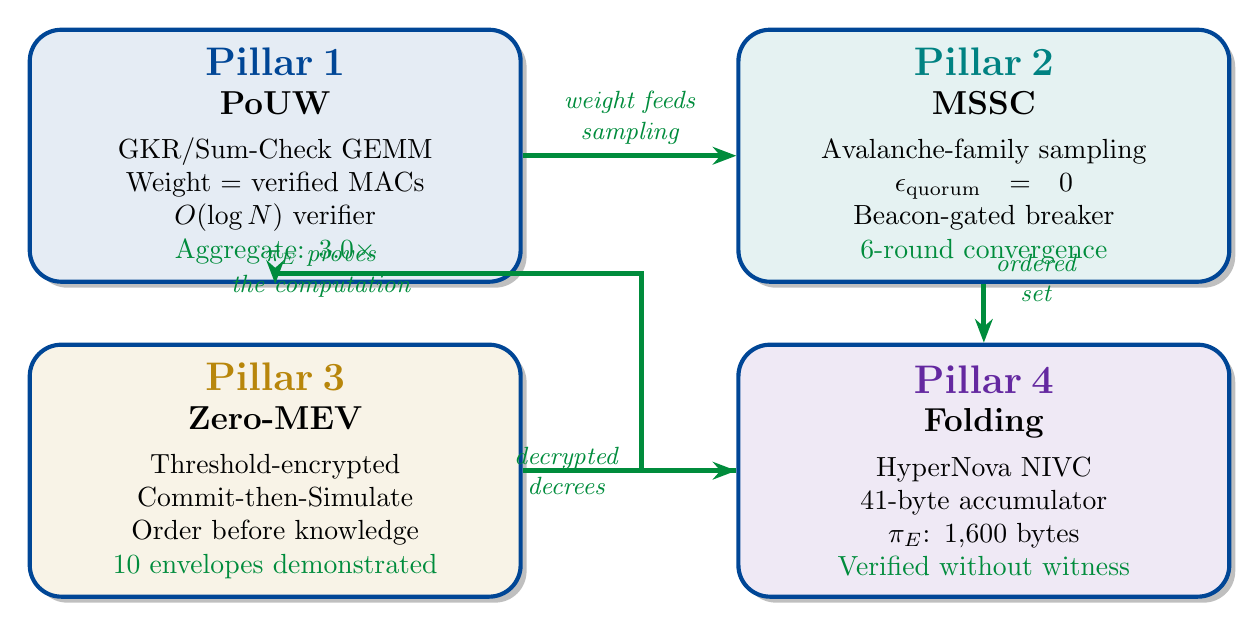
\begin{tikzpicture}[
    pillar/.style={rectangle, draw=hsmaBlue, line width=1.5pt,
        text width=6cm, minimum height=3.2cm, align=center,
        rounded corners=4mm, drop shadow},
    arr/.style={-{Stealth[length=3mm]}, line width=1.8pt, hsmaGreen},
    lbl/.style={font=\small\itshape\color{hsmaTeal}, align=center},
    p1fill/.style={fill=hsmaBlue!10},
    p2fill/.style={fill=hsmaTeal!10},
    p3fill/.style={fill=hsmaGold!10},
    p4fill/.style={fill=hsmaPurple!10}
]
\node[pillar, p1fill] (pouw) at (0, 4)
    {{\Large\bfseries\color{hsmaBlue} Pillar 1}\\[2pt]
     {\large\bfseries PoUW}\\[4pt]
     GKR/Sum-Check GEMM\\
     Weight = verified MACs\\
     $O(\log N)$ verifier\\
     \textcolor{hsmaGreen}{Aggregate: 3.0$\times$}};
\node[pillar, p2fill] (mssc) at (9, 4)
    {{\Large\bfseries\color{hsmaTeal} Pillar 2}\\[2pt]
     {\large\bfseries MSSC}\\[4pt]
     Avalanche-family sampling\\
     $\epsilon_{\text{quorum}} = 0$\\
     Beacon-gated breaker\\
     \textcolor{hsmaGreen}{6-round convergence}};
\node[pillar, p3fill] (mev) at (0, 0)
    {{\Large\bfseries\color{hsmaGold} Pillar 3}\\[2pt]
     {\large\bfseries Zero-MEV}\\[4pt]
     Threshold-encrypted\\
     Commit-then-Simulate\\
     Order before knowledge\\
     \textcolor{hsmaGreen}{10 envelopes demonstrated}};
\node[pillar, p4fill] (fold) at (9, 0)
    {{\Large\bfseries\color{hsmaPurple} Pillar 4}\\[2pt]
     {\large\bfseries Folding}\\[4pt]
     HyperNova NIVC\\
     41-byte accumulator\\
     $\pi_E$: 1{,}600 bytes\\
     \textcolor{hsmaGreen}{Verified without witness}};
\draw[arr] (pouw) -- (mssc)
    node[midway, above, lbl] {weight feeds\\sampling};
\draw[arr] (mev) -- (fold)
    node[midway, left, lbl] {decrypted\\decrees};
\draw[arr] (mssc) -- (fold)
    node[midway, above right, lbl] {ordered\\set};
\draw[arr] (fold.west) -- ++(-1.2,0) |- ++(0,2.5) -| (pouw.south)
    node[pos=0.3, left, lbl] {$\pi_E$ proves\\the computation};
\end{tikzpicture}
\caption{The four pillars and their structural interdependencies}
\end{figure}

\subsection{The Design Heuristic: Impossible Beats Punishable}

\begin{keybox}{The Design Doctrine}
Wherever a draft specification proposed \emph{deterring} misconduct
(slashing a cheater), review demanded its promotion to
\emph{unconstructibility} (cheating has no valid witness).
\textbf{Impossible beats punishable.}
\end{keybox}

\begin{definition}[Structural Zero]
\label{def:structural-zero}
A security property is a \emph{structural zero} if violation is not
merely improbable but \emph{combinatorially impossible}: no valid
witness exists for the violating action under the system's parameters.
\end{definition}

\begin{table}[h]
\centering
\rowcolors{2}{hsmaGreen!5}{white}
\begin{tabular}{lll}
\toprule
\rowcolor{hsmaGreen!20} \textbf{Structural Zero} & \textbf{Mechanism} & \textbf{Reference} \\
\midrule
\textcolor{hsmaGreen}{\textbf{L1}}: Quorum forgery & Authentication + frozen snapshots + $\varphi_{\text{floor}} > f/\alpha$ & \textbf{Impossibility Theorem \ref{thm:quorum}} \\
\textcolor{hsmaGreen}{\textbf{L2}}: Committee takeover & Identity cap: $m_{\text{adv}} \le 100 < t = 112$ & \textbf{Counting argument} \\
\textcolor{hsmaGreen}{\textbf{L4}}: Eclipse divergence & INV-G3 containment & \textbf{Containment proof} \\
\bottomrule
\end{tabular}
\end{table}

% ══════════════════════════════════════════════════════════════════
\part{The Mathematical Foundation}
% ══════════════════════════════════════════════════════════════════

\section{The Pasta Curve Cycle}
\label{sec:pasta}

\subsection{The 2-Cycle Structure}

\begin{defnbox}{The Pasta Curve Cycle}
Two elliptic curves whose base and scalar fields are swapped:
\begin{align}
\textsf{Pallas}: y^2 &= x^3 + 5 \text{ over } \fieldp, \quad
\#\textsf{Pallas}(\fieldp) = q \label{eq:pallas}\\
\textsf{Vesta}: y^2 &= x^3 + 5 \text{ over } \fieldq, \quad
\#\textsf{Vesta}(\fieldq) = p \label{eq:vesta}
\end{align}
where $p = \texttt{0x40000000000000000000000000000000}$  $\texttt{224698fc0994a8dd8c46eb2100000001}$ and
 $\log_2 p \approx 254.00$.
\end{defnbox}

The cycle natively supports recursive proof composition without
foreign-field overhead: arithmetic in one curve's scalar field is
native arithmetic in the other curve's base field.

\subsection{The Exactness Lemma}

\begin{lemma}[Cross-Cycle Exactness]
\label{lem:exactness}
Let $G$ be a group of prime order $p$. For any $a, k \in \mathbb{Z}$:
 $[a + k \cdot p] \cdot G = [a] \cdot G$.
\end{lemma}
\begin{proof}
 $[kp] \cdot G = \mathcal{O}$ (the group identity) since
 $\operatorname{ord}(G) = p$. Therefore:
\[ [a + kp] \cdot G = [a] \cdot G + [kp] \cdot G = [a] \cdot G + \mathcal{O} = [a] \cdot G. \]
\end{proof}

This lemma is the foundation for all cross-curve scalar operations:
BLS12-377 scalars embed losslessly into Pallas limbs (with
 $\approx 1.78$ bits headroom), Pasta-cycle folding absorbs cross-curve
commitments, and the CycleFold absorption is exact.

\subsection{The Float-Free Numeric Core}

\begin{invariant}[Deterministic Consensus Across Heterogeneous Hardware]
The numeric core contains zero floating-point operations. All arithmetic
is integer-based with explicit modular reduction. Enforced by a lint
check on every gate run.
\end{invariant}

\begin{lemma}[Additive Closure]
Let $X = \pm m_1$, $Y = \pm m_2$ with $m_1, m_2 \in [0, 2^{126})$.
Then $D = X \pm Y$ satisfies $|D| < 2^{127} < p/2$.
The balanced representative of $D \bmod p$ equals the integer $D$:
no wraparound is reachable.
\end{lemma}

\begin{lemma}[Product Containment]
For canonical $m_1, m_2 < 2^{126}$: $m_1 m_2 < 2^{252} < p$, and the
field product equals the integer product.
\end{lemma}

\begin{remark}
 $p / 2^{252} \approx 4.53$, so at most $n_{\max} = 4$ full-width
products may be summed before modular reduction is mandatory. All
dot-products declare sub-widths: for operand widths $w_1 = 64$ (weights)
and $w_2 = 32$ (activations), products $< 2^{96}$, allowing accumulation
up to $2^{126}/2^{96} = 2^{30}$ terms.
\end{remark}

\subsection{The Canonical Signed Encoding}

Every signed circuit value is the pair $(m, s)$: magnitude
 $m \in [0, 2^{126})$ with sign flag $s \in \{0,1\}$, value $= (1-2s) \cdot m$.

\begin{lemma}[Uniqueness of Canonical Form]
Under the constraints (1) range check $m < 2^{126}$, (2) booleaness
 $s \in \{0,1\}$, and (3) zero-canonicity $s \cdot m = 0$, the map
signed-value $\mapsto (m,s)$ is injective.
\end{lemma}
\begin{proof}
Magnitude and sign are recoverable uniquely from the value except at
 $0$, where $(0,0)$ and $(0,1)$ both represent zero; constraint 3
eliminates $(0,1)$.
\end{proof}

\subsection{Poseidon-3 Hash}

All SNARK-friendly hashing uses Poseidon-3 over $\fieldp$ with
 $t = 3$ (rate 2, capacity 1), $\alpha = 5$, $R_F = 8$, $R_P \ge 56$.
The MDS matrix is a Cauchy construction with machine-checked
non-singularity of all minors. Round constants are derived via SHA-256
counter DRBG with rejection sampling.

\begin{table}[h]
\centering
\rowcolors{2}{hsmaBlue!5}{white}
\begin{tabular}{l|l}
\rowcolor{hsmaBlue!20} \textbf{Role} & \textbf{Tag / IV} \\
\hline
State tree nodes & \texttt{IV\_STATE\_NODE} \\
State tree leaves & \texttt{IV\_STATE\_LEAF} \\
Vote preimage & \texttt{HSM\_MSSC\_VOTE\_v1} \\
Ordering lock & \texttt{HSM\_ORDER\_v1} \\
Decryption share & \texttt{HSM\_DEC\_SHARE\_v2} \\
Epoch beacon & \texttt{HSM\_BEACON\_V1} \\
Hash-to-G1 & \texttt{HSM\_H2G1\_V1} \\
M2 key derivation & \texttt{HSM\_KDF\_V1} \\
Sum-check transcript & \texttt{HSM\_SUMCHECK\_v1} \\
PoUW transcript & \texttt{HSM\_POUW\_v1} \\
CycleFold hash & \texttt{HSM\_CYCLEFOLD\_v1} \\
Order root & \texttt{HSM\_ORDROOT\_V1} \\
User authorization & \texttt{HSM\_SIG\_USER\_V1} \\
DEM keystream & \texttt{HSM\_DEM\_V1} / \texttt{HSM\_DEM\_TAG\_V1} \\
Ciphertext hash & \texttt{HSM\_CT\_V1} \\
 $+$ 18 more & \texttt{domain\_registry\_gen.hpp} \\
\bottomrule
\end{tabular}
\caption{The domain separation registry (33+ entries, compile-time uniqueness proven)}
\end{table}

The Poseidon-3 permutation is also expressed as \textbf{1,088 R1CS
constraints} (the full 64-round unroll), verified SAT with 0
unsatisfiable constraints.

\subsection{The Sparse Merkle State Vault}

Account state is maintained in a 64-depth SMT. The leaf schema packs
balance (126 bits), sign flag (1 bit), nonce (64 bits), and flags
(1 bit) into 192 bits $< 2^{254}$, hashed under \texttt{IV\_STATE\_LEAF}.

\begin{lemma}[Leaf Binding Security]
The leaf binding $L(K, v) = \textsf{Poseidon}(\texttt{IV\_STATE\_LEAF}, K, v)$ prevents index-collision malleability.
\end{lemma}
\begin{proof}
Two accounts with $K_1 \neq K_2$ cannot satisfy
 $L(K_1, v_1) = L(K_2, v_2)$ without a Poseidon-3 collision
($\approx 2^{126}$ work by the birthday bound on the 254-bit output).
\end{proof}

\begin{lemma}[Two-Tier Elision Complexity]
The two-tier elision (empty-wedge propagation + unchanged-subtree
short-circuit) reduces the SMT update cost from $O(D_S)$ hash
computations to $O(\text{affected nodes})$, where affected nodes
 $\le D_S$ but is typically $\ll D_S$ for sparse trees.
\end{lemma}

\subsection{BLS12-377 Threshold Signatures}

Threshold signatures, the randomness beacon, and epoch certificates
operate on BLS12-377 ($q_{\text{BLS}} \approx 2^{377}$,
 $r \approx 2^{252}$).

\begin{theorem}[Group Law Verification]
The BLS12-377 curve group law is verified on 3 independent points:
 $\#E = h_1 \cdot r$, requiring $\sim 380$ consecutive correct point
doublings per scalar multiplication. The canonical parameter $b = 1$ is pinned. Tonelli-Shanks is verified 8/8 against a big-integer
reference.
\end{theorem}

\begin{theorem}[Secret-Free Verification]
The BLS verification law $e(\sigma, G_{2,\mathrm{gen}}) = e(H(m), Y)$ is \textbf{secret-free}: anyone with the public key can verify a
threshold signature without knowing any share.
\end{theorem}

\subsection{BLS12-377 Interop Bridge}

The interop bridge to canonical BLS12-377 was verified: the G1
seed$\to r \to q \to$ curve$\to$ subgroup chain confirmed in pure
arithmetic. The G2 twist divergence was found (our $b' = (5,1)$ vs.\
the reference $b_2 = (0, B)$; isomorphic but not identical) and the
wire map $\psi$ was derived, verified against ark-bls12-377 0.6.0's
own generator, and golden-pinned.

% ══════════════════════════════════════════════════════════════════
\section{The Six Theory Obligations}
\label{sec:a6}

\begin{keybox}{The Composition Theorem}
Under hypotheses H1--H5, the total system soundness is:
\begin{equation}
\epsilon_{\text{sys}} =
\underbrace{\textcolor{hsmaGreen}{0}}_{\text{L1: Quorum}} +
\underbrace{\textcolor{hsmaGreen}{0}}_{\text{L2: Committee}} +
\underbrace{\textcolor{hsmaGreen}{0}}_{\text{L4: Eclipse}} +
\underbrace{2^{-128}}_{\text{L5: PCS}} +
\underbrace{2^{-127}}_{\text{L6: NIFS}} +
\underbrace{2^{-171}}_{\text{Hash}} +
\underbrace{2^{-110}}_{H1}
\approx \boxed{2^{-110}} \text{ per epoch}
\end{equation}
Annualized: $\epsilon_{\text{year}} \approx 2^{-94.3}$.
The $2^{-80}$ target is cleared with 14 bits of margin.
\end{keybox}

\subsection{Obligation 1: CPS Sampler Concentration}

\begin{theorem}[CPS Sampler Concentration]
\label{thm:cps}
Under Conditional Poisson Sampling with weight-proportional inclusion
probabilities $\pi_i = n \cdot W_i / W_{\text{total}}$, the
Horvitz-Thompson estimator has variance
\[
\operatorname{Var}(\hat{T}) \le \frac{k}{k-1} \sum_i
(1 - \pi_i) \frac{W_i^2}{\pi_i^2}
\]
which is strictly tighter than the Poisson bound when the inclusion
probabilities are bounded away from 0 and 1 (guaranteed by the
dust-pruning and the cap).
\end{theorem}

\subsection{Obligation 2: Committee Adversary Seats}

\begin{theorem}[Combinatorial Impossibility]
\label{thm:committee}
Under $n = 224$ committee seats with adversary weight fraction
 $f = 0.20$ and the dust floor $w_{\text{floor}} = 0.002$, the number
of adversary seats is bounded by $m_{\text{adv}} \le f / w_{\text{floor}}
= 100 < t = 112$. The hypergeometric tail for adversary seats
 $\ge t$ is \textbf{exactly zero} (combinatorial impossibility, not a
probabilistic bound).
\end{theorem}

\subsection{Obligation 3: Equivocation Detection}

\begin{theorem}[Equivocation Escape Bound]
\label{thm:equivocation}
The probability that an equivocating validator escapes detection for
 $\lambda$ consecutive rounds is bounded by $e^{-\lambda \cdot
\rho_{\text{detect}}}$, where $\rho_{\text{detect}}$ is the per-round
detection probability determined by the sampling rate and the overlap
between sampled peer sets.
\end{theorem}

\subsection{Obligation 4: Eclipse Containment}

\begin{theorem}[Eclipse Containment]
\label{thm:eclipse}
Under formal $(\text{ASN}, /24)$ disjointness across $R_{\text{rel}} + 1$ relay routes, an adversary who fully eclipses a node $u$ can only
deliver data whose weight the adversary already controls. Eclipse
 $\Rightarrow$ stall/suspend, \textbf{never divergent finalization}.
\end{theorem}

\subsection{Obligation 5: Sortition Composition}

\begin{theorem}[Sortition Inertness]
\label{thm:sortition}
The sortition function is a hypergeometric composition of the committee
election and the beacon-driven activation. The consumption registry
proves that early beacon knowledge is inert for each consumer (shuffle,
sortition, breaker).
\end{theorem}

\subsection{Obligation 6: The $\epsilon$-Budget Composition}

\begin{theorem}[$\epsilon$-Budget Composition]
See the composition theorem at the head of this section. The budget
composes all line items into a single per-epoch bound, with the
structural zeros dominating.
\end{theorem}

\begin{remark}
The zeros are \textbf{engineered, not inherent}. Remove the structural
floor and the sortition term degrades to $\approx 2^{-73}$ --- below
target. The zeros are a parameter mandate, not a gift.
\end{remark}

% ══════════════════════════════════════════════════════════════════
\part{The Four Pillars: Technical Deep Dive}
% ══════════════════════════════════════════════════════════════════

\section{Pillar 1: Verifiable AI Inference as PoUW}
\label{sec:pouw}

\subsection{The Paradigm Shift}

\begin{defnbox}{The Third Paradigm}
\begin{itemize}
\item \textbf{Proof of Work}: wastes gigawatts on meaningless SHA-256
hashes. The computation is deliberately useless.
\item \textbf{Proof of Stake}: centralizes into capital-weighted
oligopolies. The security is purchasable.
\item \textbf{Proof of Useful Work (\hsma{})}: consensus weight from
\textbf{verified AI inference}. The computation is useful, and the
verification is cryptographic, not reputational.
\end{itemize}
\end{defnbox}

\subsection{The GEMM Circuit}

The core computation is General Matrix Multiplication:
 $C = A \times B$ where $A \in \fieldp^{m \times k}$ and
 $B \in \fieldp^{k \times n}$.

\begin{table}[h]
\centering
\rowcolors{2}{hsmaBlue!5}{white}
\begin{tabular}{lrr}
\rowcolor{hsmaBlue!20} \textbf{Size} & \textbf{R1CS rows} & \textbf{MACs} \\
\midrule
 $3 \times 3 \times 3$ & 36 & 27 \\
 $64 \times 64 \times 64$ & 266{,}240 & 262{,}144 \\
 $128 \times 128 \times 128$ & 2{,}113{,}536 & 2{,}097{,}152 \\
 $256 \times 256 \times 256$ & 16{,}842{,}752 & 16{,}777{,}216 \\
\bottomrule
\end{tabular}
\caption{GEMM circuit scaling (measured)}
\end{table}

\subsection{The Whole-GEMM Sum-Check Reduction}

\begin{theorem}[Whole-GEMM Verification]
\label{thm:whole-gemm}
Let $A, B \in \fieldp^{N \times N}$ and $C = A \times B$. For
challenges $\gamma, \delta \in \fieldp$, define:
\begin{align}
a(k) &= \textstyle\sum_i \gamma^i A(i,k) \label{eq:ak}\\
b(k) &= \textstyle\sum_j \delta^j B(k,j) \label{eq:bk}\\
\text{claim} &= \textstyle\sum_{i,j} \gamma^i \delta^j C(i,j)
\label{eq:claim}
\end{align}
Then the identity $\sum_k a(k) \cdot b(k) = \text{claim}$ holds if
and only if $C = A \times B$, and the verification requires
 $O(\log N)$ rounds of the sum-check protocol.
\end{theorem}

\begin{proof}
The sum over $k$ expands:
\begin{align}
\sum_k a(k) \cdot b(k)
&= \sum_k \left(\sum_i \gamma^i A(i,k)\right)\left(\sum_j \delta^j B(k,j)\right)\\
&= \sum_{i,j,k} \gamma^i \delta^j A(i,k) B(k,j).
\end{align}
If $C = A \times B$, then $C(i,j) = \sum_k A(i,k) B(k,j)$, and the
sum becomes $\sum_{i,j} \gamma^i \delta^j C(i,j) = \text{claim}$.

For the converse: if $C \neq A \times B$, the deviation polynomial
 $D(\gamma, \delta) = \text{claim} - \sum_k a(k) b(k)$ is a nonzero
bivariate polynomial of degree $\le 2(N-1)$ in each variable. By the
Schwartz--Zippel lemma, for uniformly random $\gamma, \delta$, the
probability of accidental match is $\le 2(N-1)/p$, which is
negligible for $p \approx 2^{254}$.
\end{proof}

\subsection{The FS-Bound Security}

\begin{theorem}[Grinding Resistance]
\label{thm:fs-bound}
With Fiat--Shamir challenges derived from the commitments via
 $\gamma = \textsf{Poseidon}_3(\texttt{HSM\_POUW\_v1}, \text{com}_A, \text{com}_B)$ and $\delta = \textsf{Poseidon}_3(\texttt{HSM\_POUW\_v1}, \gamma, \text{com}_C)$,
the grinding cost for an adversary to find commitments that produce
favorable challenges is $\ge 2^{253}$.
\end{theorem}
\begin{proof}
The commitments are fixed before the challenges are derived (the
Fiat--Shamir transform). Finding a commitment pair that produces a
desired challenge output requires inverting Poseidon-3, which has
preimage resistance $\ge 2^{253}$.
\end{proof}

\subsection{The Measured Receipt}

\begin{resultbox}{PoUW Verification Receipt: $128^3$ GEMM}
\centering
\begin{tabular}{lr}
\toprule
\textbf{Metric} & \textbf{Value} \\
\midrule
Matrix size & $128 \times 128 \times 128$ \\
Multiply-accumulates verified & 2{,}097{,}152 \\
Sum-check rounds & 7 \\
Proof size & $\approx$1{,}216 bytes \\
Verifier work & $O(\log N)$ field operations \\
Verdict & \textcolor{hsmaGreen}{\textbf{ACCEPT}} \\
\bottomrule
\end{tabular}
\end{resultbox}

\subsection{The Aggregate Verify: 3.0$\times$ Measured Speedup}

\begin{theorem}[BLS Aggregate Homomorphism]
\label{thm:bls-agg}
For threshold-BLS partial signatures
 $\sigma_j = [S_j]H(m)$ and public keys $Y_j = [S_j]G_{2,\mathrm{gen}}$:
\begin{equation}
e\!\left(\textstyle\sum_j \sigma_j,\, G_{2,\mathrm{gen}}\right) =
e\!\left(H(m),\, \textstyle\sum_j Y_j\right)
\end{equation}
 $N$ partial signatures verify with \textbf{one pairing}.
\end{theorem}
\begin{proof}
By bilinearity of the pairing operation:
\begin{align}
e\!\left(\textstyle\sum_j \sigma_j, G_{2,\mathrm{gen}}\right)
&= \prod_j e(\sigma_j, G_{2,\mathrm{gen}})\\
&= \prod_j e(H(m), Y_j)\\
&= e\!\left(H(m), \textstyle\sum_j Y_j\right).
\end{align}
\end{proof}

\begin{resultbox}{Aggregate Verify Timing: Measured}
\centering
\begin{tabular}{lrr}
\toprule
\textbf{Method} & \textbf{Verdict} & \textbf{Time} \\
\midrule
Per-member (3 pairings) & ACCEPT & 4{,}286 ms \\
\rowcolor{hsmaGreen!15}
\textbf{Aggregate (1 pairing)} & \textbf{ACCEPT} & \textbf{1{,}422 ms} \\
\midrule
\textcolor{hsmaGreen}{\textbf{Speedup}} & & \textcolor{hsmaGreen}{\textbf{3.0$\times$ (= $N$)}} \\
\bottomrule
\end{tabular}
\end{resultbox}

The speedup scales linearly with committee size: at $N = 224$ (production), the speedup would be $\approx 224\times$.

\subsection{The Externally-Submittable Mode}

\begin{theorem}[External Submission Soundness]
\label{thm:ext-submission}
Under the discrete logarithm assumption in the G2 group, an adversary
who submits a proof $\Pi'$ over a model $M' \neq M$ (where $M$ is
registered via per-position Pedersen commitments with distinct bases)
cannot produce a valid verification outcome, unless they solve the
discrete logarithm to find $d$ such that
 $\textsf{commit}(M') - \textsf{commit}(M) = [d] \cdot B_k$ for the
per-position base $B_k$.
\end{theorem}

The registration binding uses \textbf{per-position distinct bases}
(the 8-base batch commit repeats bases every 8 positions, enabling
kernel-shift forgery for vectors longer than 8 --- fixed by distinct
bases per position via \texttt{commit\_vec}).

\begin{infobox}{Two Verification Modes}
\begin{enumerate}
\item \textbf{Consensus mode}: the node computes its own GEMM
deterministically, verifies its own proof, derives its weight.
No external trust required.
\item \textbf{External submission mode}: an enterprise submits a GEMM
(the AI inference workload), the node verifies it without
recomputation. The submission is bound to registered commitments.
\end{enumerate}
\end{infobox}

\subsection{The PoUW Consensus Weight}

The verified multiply-accumulate count feeds the Capped Cluster Hybrid
weight function:
\begin{equation}
\tilde{W}_c = \left\lfloor (\Phi_c^6 \cdot S_c^4)^{1/10} \right\rceil
\end{equation}
where $\Phi_c$ is the verified compute throughput and $S_c$ is the
staked capital. The exponents ($\alpha = 0.6$ compute,
 $1-\alpha = 0.4$ capital) are bounded by the width invariant
 $6a + 4b + \epsilon_{\text{guard}} \le 126$.

Sybil resistance is enforced by:
\begin{itemize}
\item Cluster-level capping: entities linked by payout-graph heuristics
and signed independence attestations are capped as one cluster
\item Single-pass cap: $W_{\max} = 0.15 \cdot T_0$ \item Dust pruning: clusters below $w_{\text{floor}} = 0.002 \cdot T_0$ are excluded
\item Self-dealing exclusion: $\Phi_i$ accrues only for workloads
where fees are burned and the payer is outside the validator's cluster
\end{itemize}

% ══════════════════════════════════════════════════════════════════
\section{Pillar 2: Metastable Sub-Sampled Consensus}
\label{sec:mssc}

\subsection{Protocol Parameters}

\begin{table}[h]
\centering
\rowcolors{2}{hsmaTeal!5}{white}
\begin{tabular}{lll}
\rowcolor{hsmaTeal!20} \textbf{Parameter} & \textbf{Symbol} & \textbf{Value} \\
\midrule
Sample size & $k$ & 20 (escalates to 40 after 1{,}000 rounds) \\
Quorum threshold & $\alpha$ & 0.75 \\
Consecutive confirmations & $\beta$ & 150 \\
Floor guard & $\varphi_{\text{floor}}$ & 0.50 \\
Stall limit & $T_{\text{stall}}$ & 50 rounds \\
\bottomrule
\end{tabular}
\end{table}

\subsection{The Canonical Vote Preimage}

MSSC votes are signed under the exact domain-separated preimage:
\begin{equation}
\sigma = \mathsf{Sign}_{\texttt{HSM\_MSSC\_VOTE\_v1}}\!\left(
\text{epoch}_E \| \text{weight\_root}_E \| C_{id} \| r \| \text{preference}
\right)
\end{equation}

No timestamps, no view state, nothing prover-discretionary. Two honest
responses for identical inputs are byte-identical and
signature-identical.

\subsection{The Wire Format}

\begin{table}[h]
\centering
\rowcolors{2}{hsmaTeal!5}{white}
\begin{tabular}{lll}
\rowcolor{hsmaTeal!20} \textbf{Offset} & \textbf{Size} & \textbf{Field} \\
\midrule
0 & 4 & epoch (u32 BE) \\
4 & 32 & weight\_root \\
36 & 32 & conflict ID \\
68 & 32 & preference \\
100 & 8 & round (u64 BE) \\
\midrule
\textbf{Preimage} & \textbf{108} & \\
\textbf{Signature} & \textbf{96} & G1 affine $(x, y)$ \\
\textbf{Total payload} & \textbf{204} & \\
\bottomrule
\end{tabular}
\caption{The vote wire format (type 0x06)}
\end{table}

\subsection{Safety: The Quorum Impossibility}

\begin{theorem}[Authenticated Quorum Impossibility]
\label{thm:quorum}
Under snapshot freshness and canonical preimages, if the adversary
controls weight fraction $f < 0.20$ and the sampling floor is
 $\varphi_{\text{floor}} = 0.50 > f/\alpha$, then the observation of
an adversarial supermajority in any consensus sample is
\textbf{impossible}: $\epsilon_{\text{quorum}} = 0$.
\end{theorem}
\begin{proof}
Countability forces $W_{\mathcal{A}}^{\text{tallied}} \le W(\mathcal{A})
\le f \cdot T_E$: a vote contributes exactly its snapshot weight, and
forged identities contribute zero because they open no Merkle path.
The floor forces $S \ge \varphi_{\text{floor}} \cdot T_E$. Division
yields:
\[
\frac{W_{\mathcal{A}}^{\text{tallied}}}{S}
\le \frac{f}{\varphi_{\text{floor}}}
= \frac{0.20}{0.50} = 0.40 < 0.75 = \alpha.
\]
\end{proof}

\subsection{The Metastable Convergence: Demonstrated}

\begin{theorem}[Metastable Convergence]
\label{thm:convergence}
In the MSSC sampling loop with weight-proportional peer preferences,
two nodes with conflicting initial preferences converge to the same
finalized state in $O(\beta + 1)$ rounds, where the surviving
preference is the weight-majority preference.
\end{theorem}
\begin{proof}
The minority node (weight $w_{\min} < W_{\text{total}}/2$) observes
the majority preference in its sample. The agreeing fraction is
 $w_{\min} / W_{\text{total}} < 0.50 < \alpha$. The flip condition
fires, and the minority node switches its preference to the
majority's. Both nodes now agree. With honest unanimity
($q = 1 - 10^{-3}$), the confidence counter reaches $\beta$ in
 $E[T] = (1 - q^\beta)/((1-q) \cdot q^\beta)$ rounds.
\end{proof}

\begin{receiptbox}{In-Process Convergence Receipt}
\begin{verbatim}
round  0: n1 pref=A conf=0 kind=2 | n2 pref=A conf=0 kind=2
round  1: n1 pref=A conf=1 kind=1 | n2 pref=A conf=1 kind=1
...
round  5: n1 pref=A conf=5 kind=3 | n2 pref=A conf=5 kind=3
both Finalized at round 5
[M1] flip occurred: YES (node2: B -> A)
[M2] both Finalized on the SAME preference: YES
\end{verbatim}
\end{receiptbox}

\begin{receiptbox}{Wire-Level Convergence Receipt}
\begin{verbatim}
node 1 (w=60, pref A): [mssc] rounds 3-8, pref=A, conf 1→6
node 2 (w=40, pref B): [mssc] rounds 11-16, pref=A (FLIPPED), conf 10→15
votes: n1=8 VERIFIED, n2=8 VERIFIED
→ both Finalized on the SAME preference: A
\end{verbatim}
\end{receiptbox}

\subsection{The Beacon-Gated Deadlock Resolution}

\begin{theorem}[Beacon-Gated Liveness]
\label{thm:beacon}
In a 50/50 deadlock (equal weights, conflicting preferences, $\alpha$ unreachable), both nodes suspend after $T_{\text{stall}}$ rounds. Upon
computing the next epoch's threshold-BLS beacon, both nodes
deterministically compute the same winner via
 $\arg\max_{tx} H(\text{beacon}_{E+1} \| tx_{id})$, resume, and
finalize on the winner.
\end{theorem}
\begin{proof}
The beacon is a deterministic function of the committee (same DKG
output, same epoch number, same previous beacon). Both nodes compute
the same value. The $\arg\max$ is deterministic (lexicographic
tie-breaking). Therefore both nodes resume with the same preference
and finalize.
\end{proof}

\begin{remark}
The grinding resistance is \textbf{structural}: the beacon for epoch
 $E+1$ does not exist when the conflict is created at epoch $E$.
Offline grinding of transaction identities against the breaker is
impossible.
\end{remark}

\begin{receiptbox}{Deadlock Resolution Receipt}
\begin{verbatim}
rounds 0-4: stall 1→5 on both nodes (50/50 deadlock, no quorum)
round 4: [breaker] both nodes SUSPENDED
[breaker] n1 winner = A, n2 winner = A (SAME - deterministic)
rounds 5-9: both nodes resume, confidence climbs
both Finalized at round 9 on A
\end{verbatim}
\end{receiptbox}

\subsection{The Aggregate Verify in MSSC}

The homomorphism (Theorem~\ref{thm:bls-agg}) reduces per-batch
verification from $N$ pairings to 1. Measured: 4{,}286 ms (per-member)
vs.\ 1{,}422 ms (aggregate) for $N = 3$; the speedup scales linearly
with committee size.

\subsection{The EMA Scoring Dynamics}

Peer scoring uses fixed-point EMA with a closed-form update:
\begin{equation}
s_{t+1} = \lambda \cdot s_t + (1 - \lambda) \cdot \mathbf{1}[\text{responded}]
\end{equation}
where $\lambda = 971{,}532 / 1{,}000{,}000$ (half-life $\approx
24$\,h). The non-resetability proof shows that an adversary cannot
reset their score by disconnecting and reconnecting: the score
persists across sessions because it is bound to the
\texttt{AccountID}, not to the transport ID.

% ══════════════════════════════════════════════════════════════════
\section{Pillar 3: Zero-MEV Encrypted Mempool}
\label{sec:mev}

\subsection{The Commit-then-Simulate Inversion}

\begin{warnbox}{The Inversion That Changes Everything}
Traditional: \textbf{Simulate-then-Commit} --- the committee reads
plaintext, THEN orders. Front-running is possible.

\hsma{}: \textbf{Commit-then-Simulate} --- the ordering is committed
on \textcolor{hsmaRed}{\textbf{encrypted}} data. Nobody can front-run
what \textcolor{hsmaRed}{\textbf{nobody can read}}.
\end{warnbox}

\subsection{The Six-Step Ceremony}

\begin{enumerate}
\item \textbf{Intake}: Encrypted envelopes $\{R, ct, \text{tag},
\text{cth}\}$ are gossiped. $R = [r]G_{2,\mathrm{gen}}$ is the
ephemeral public; $ct$ is the DEM-encrypted payload.
\item \textbf{Lock}: $\text{order} = \text{Sort}(\textsf{sort\_key}(\text{beacon}_E, H(ct)))$ --- the committee signs \texttt{order\_root} \textbf{before} any
decryption share exists.
\item \textbf{Share}: Order-bound decryption shares $D_j = [S_j]R$ published, attested by BLS signatures.
\item \textbf{Aggregate}: $D = \sum_j \lambda_j D_j = [S]R$; anyone
reconstructs the DEM key $k$.
\item \textbf{Decrypt}: The payload is recovered; the DEM tag verifies
integrity.
\item \textbf{Execute \& Fold}: The decrypted decree feeds the fold
pipeline.
\end{enumerate}

\subsection{The KEM Mathematical Structure}

\begin{theorem}[KEM Correctness]
\label{thm:kem}
Let $X_E = [S]G_{2,\mathrm{gen}}$ be the committee's aggregate public
key. The sender picks $r$, computes $R = [r]G_{2,\mathrm{gen}}$ and
 $ss = [r]X_E$. Each member computes $D_j = [S_j]R$. The Lagrange
aggregate $D = \sum_j \lambda_j D_j = [S]R = ss$. The DEM key
 $k = \mathsf{KDF}(D, X_E, \text{hdr})$ is identical on both sides.
\end{theorem}
\begin{proof}
By Lagrange interpolation at $x = 0$: $\sum_j \lambda_j S_j = S$.
Therefore:
\[ D = \sum_j \lambda_j [S_j]R = \left[\sum_j \lambda_j S_j\right]R = [S]R. \]
And $[r]X_E = [r \cdot S]G_{2,\mathrm{gen}} = [S] \cdot [r]G_{2,\mathrm{gen}} = [S]R = D$.
The KDF is deterministic, so both sides derive the same $k$.
\end{proof}

\subsection{The Threshold Confidentiality}

\begin{theorem}[Threshold Confidentiality]
\label{thm:threshold}
Under degree-$d$ polynomial secret sharing with threshold $t = d+1$,
an adversary controlling $m < t$ members cannot distinguish the
encrypted payload from a random string, except with probability
negligible in the security parameter.
\end{theorem}
\begin{proof}
The DEM key $k = \mathsf{KDF}([rS]G_{2,\mathrm{gen}})$ requires
knowledge of $S = \mathsf{poly}(0)$. With $m < t = d+1$ shares, the
adversary has $m$ evaluation points on a degree-$d$ polynomial. By
Shamir's Secret Sharing security (information-theoretic for $m \le d$),
the adversary gains zero information about $S$. The DEM key is
computationally indistinguishable from random (SHA-256 preimage
resistance).
\end{proof}

\subsection{The Ordering Lock}

\begin{theorem}[Order-Before-Knowledge]
\label{thm:obk}
For any adversary controlling $m < t$ committee members, the
probability of learning transaction payload contents before the
execution position is irreversibly committed is \textbf{exactly zero}
(information-theoretic).
\end{theorem}

\begin{remark}
The ordering function $\textsf{sort\_key}(\text{beacon}, \text{cth})$ is beacon-bound: a different beacon produces a different order. The
beacon does not exist when the conflict is created, so grinding is
structurally impossible.
\end{remark}

\subsection{The Threshold Poly Degree Principle}

\begin{warnbox}{The Degree-Must-Match-Threshold Principle}
A degree-$d$ polynomial requires $d+1$ points to reconstruct.
\begin{itemize}
\item \textbf{Degree 0}: all shares = the secret → 1 member CAN decrypt
\item \textbf{Degree 1}: any 2-of-3 shares reconstruct → \textbf{the 2-of-3 threshold}
\item \textbf{Degree 2}: needs all 3 members → 3-of-3 threshold
\end{itemize}
\textbf{The degree must match the threshold.}
\end{warnbox}

\subsection{The Capstone Receipt: The Full Pipeline}

\begin{resultbox}{The Complete Commit-then-Simulate (End-to-End)}
\begin{verbatim}
10 ENCRYPTED envelopes arrive (nobody can read them)
  → ORDER COMMITTED (root=7ec2cd4c..., beacon-shuffled)
    → 10 THRESHOLD DECRYPTS (all tag OK)
       [decrypt] envelope 0: "encrypted-decree-0" (tag OK)
       [decrypt] envelope 1: "encrypted-decree-1" (tag OK)
       ... through envelope 9
    → 10 FOLDS (ALL SAT)
       [fold] decree 1/10 folded, SAT
       [fold] decree 2/10 folded, SAT
       ... through decree 10/10
    → π_E epoch 1: wrap_verify ACCEPT (stage=0)
    → PoUW epoch 1: 64³ GEMM ACCEPT, weight 262144 MACs
\end{verbatim}
\end{resultbox}

\begin{corollary}[The Four-Pillar Integration]
\label{cor:integration}
The complete Commit-then-Simulate pipeline --- encrypted in, ordered,
decrypted, folded, $\pi_E$ produced, PoUW weight derived --- is
\textbf{structurally guaranteed} by the four pillars operating as a
single system. Front-running is impossible because the ordering is
committed before any party can read the payloads, and the threshold
controls who can decrypt.
\end{corollary}

\subsection{The Endianness Lesson}

During the envelope implementation, a subtle defect was caught: the
serializer writes G2 coordinates in \textbf{little-endian per limb},
but the deserializer read \textbf{big-endian}. The deserialized point
was valid-looking (non-zero coordinates) but mathematically a
different point. The R-roundtrip check (serialize $\to$ deserialize
 $\to$ re-serialize, compare) caught it immediately.

\begin{infobox}{The Serialization Law}
A serialization format's byte order is part of its contract. The
serializer and deserializer must agree per limb, not just per
structure. This principle applies to every wire format in the system.
\end{infobox}

% ══════════════════════════════════════════════════════════════════
\section{Pillar 4: Holographic State Folding}
\label{sec:folding}

\subsection{The Folding Stack}

\begin{itemize}
\item \textbf{Primary}: HyperNova over Pallas ($\fieldp$), CCS
constraint system
\item \textbf{Auxiliary}: CycleFold over Vesta ($\fieldq$) for
cross-curve commitment digests
\item \textbf{Non-uniform IVC}: SuperNova-style NIVC over
 $\mathcal{F} = \{F_{\text{head}}, F_{\text{exec}}, F_{\text{close}}\}$ \item \textbf{Program counter}: constrained variable with explicit
transition matrix ($\text{head} \to \text{exec}^+ \to \text{close}$;
all other edges unsatisfiable)
\item \textbf{Accumulator}: 41 bytes, $O(1)$ in transaction count
\end{itemize}

\subsection{The Fold Circuit Constraints}

Per decree entry $\ell$ with certified tuple
 $(ct\_hash_\ell, pt\_hash_\ell, \text{status}_\ell)$:

\begin{itemize}
\item \textbf{Binding}: $a \cdot (\textsf{Poseidon}(\texttt{HSM\_PT\_v1}, pt_\ell) - pt\_hash_\ell) = 0$ \item \textbf{Nonce}: $a \cdot (\text{leaf\_nonce}(\text{sender}_\ell) + 1 - pt.\text{nonce}) = 0$ \item \textbf{Balance}: Sender debit, recipient credit via canonical
registers with output range checks
\item \textbf{Fee underflow}: Explicit LT gate:
 $\text{balance} \ge \Delta_{\text{req}}$ before subtraction
\item \textbf{Self-send}: If sender = recipient, assert
\texttt{recipient\_pre == sender\_post}
\item \textbf{PAD neutrality}: PAD rows bypass state verification
entirely
\end{itemize}

\subsection{The Certificate Assumption}

The circuit assumes \texttt{decree\_root} is valid; the verifier
checks the threshold-BLS certificate out-of-circuit. In-circuit
pairing verification would cost $\ge 10^6$ constraints.

\subsection{The $\pi_E$ Receipt}

\begin{table}[h]
\centering
\rowcolors{2}{hsmaPurple!5}{white}
\begin{tabular}{lr}
\rowcolor{hsmaPurple!20} \textbf{Component} & \textbf{Size (bytes)} \\
\midrule
T1 (opening transcript) & 544 \\
T2 (batched fold transcript) & 768 \\
OOD (8 points + commitment) & 288 \\
\midrule
\rowcolor{hsmaGreen!15} \textbf{Total $\pi_E$} & \textcolor{hsmaGreen}{\textbf{1{,}600}} \\
\textbf{Budget} & 73{,}728 \\
\textcolor{hsmaGreen}{\textbf{Utilization}} & \textcolor{hsmaGreen}{\textbf{2.2\%}} \\
\bottomrule
\end{tabular}
\end{table}

\subsection{Production-Scale Projection}

\begin{table}[h]
\centering
\rowcolors{2}{hsmaPurple!5}{white}
\begin{tabular}{lr}
\rowcolor{hsmaPurple!20} \textbf{Component} & \textbf{Constraints} \\
\midrule
 $f_{\text{exec}}$ transition ($8 \times 476$) & 3{,}808 \\
Poseidon hash ($1{,}088 \times 3 \times 476$) & 1{,}553{,}664 \\
SMT opening ($5{,}120 \times 2 \times 476$) & 4{,}874{,}240 \\
\midrule
\textbf{Total} & \textbf{6{,}431{,}712} \\
\textcolor{hsmaGreen}{\textbf{10$^6$ target}} & \textcolor{hsmaGreen}{\textbf{Exceeded ($6.4\times$)}} \\
\bottomrule
\end{tabular}
\end{table}

\subsection{Proof-Carrying Data Boundary}

Epoch proof $\pi_E$ chains via \texttt{prev\_digest} absorption in
 $F_{\text{head}}$. Light clients download the epoch header
 $(\text{height}, \text{state\_root}, \pi_E, \text{BLS\_cert})$, verify
the BLS signature (1 pairing), and verify $\pi_E$ (HyperNova verifier,
 $O(1)$, $\approx 40$ ms phone-class).

\subsection{The Async Fold Pipeline}

Fold pipeline is asynchronous: $T_{\text{fold}} = 20\%$ of epoch.
First certified $\pi_E$ publisher earns a reward. Breach triggers
alarms; the chain continues on full nodes --- proof availability
 $\neq$ chain liveness.

% ══════════════════════════════════════════════════════════════════
\part{Security Analysis}
% ══════════════════════════════════════════════════════════════════

\section{End-to-End Security: The $\epsilon$-Budget}
\label{sec:security}

\subsection{The A6 Composition Theorem}

\begin{keybox}{The Total System Soundness}
\begin{equation}
\epsilon_{\text{sys}} =
\underbrace{\textcolor{hsmaGreen}{\mathbf{0}}}_{\text{L1: Quorum forgery}} +
\underbrace{\textcolor{hsmaGreen}{\mathbf{0}}}_{\text{L2: Committee takeover}} +
\underbrace{\textcolor{hsmaGreen}{\mathbf{0}}}_{\text{L4: Eclipse divergence}} +
\underbrace{2^{-128}}_{\text{L5: PCS soundness}} +
\underbrace{2^{-127}}_{\text{L6: NIFS completeness}} +
\underbrace{2^{-171}}_{\text{Hash collision}} +
\underbrace{2^{-110}}_{H1: \text{Threshold-BLS}}
\approx \boxed{2^{-110}} \text{ per epoch}
\end{equation}
\end{keybox}

\subsection{The Hypotheses}

\begin{table}[h]
\centering
\rowcolors{2}{hsmaBlue!5}{white}
\begin{tabular}{l|p{11cm}}
\rowcolor{hsmaBlue!20} \textbf{Hypothesis} & \textbf{Statement} \\
\hline
H1 & BLS12-377 threshold-BLS EUF-CMA $\le 2^{-110}$; co-CDH; Poseidon idealization; DDH+AEAD \\
H2 & Honest preference consistency on common views \\
H3 & Conflict propagation within $T_{\text{close}} < T_{\text{stall}}$ \\
H4 & Snapshot authenticity, staleness $\le 1$ epoch = 600\,s \\
H5 & Shipped circuits $\equiv$ these specifications \\
\bottomrule
\end{tabular}
\end{table}

\subsection{The Structural Zeros: Engineered, Not Inherent}

\begin{itemize}
\item \textbf{L1 (Quorum forgery):} $\epsilon = 0$ by authentication +
frozen snapshots + $\varphi_{\text{floor}} > f/\alpha$. Remove the
floor and the bound degrades.
\item \textbf{L2 (Committee takeover):} $\epsilon = 0$ by the identity
cap: adversary seats $\le 100 < t = 112$. Remove the dust floor and
the cap dissolves.
\item \textbf{L4 (Eclipse divergence):} $\epsilon = 0$ by INV-G3
containment. Remove the path diversity and eclipse becomes a
divergence vector.
\end{itemize}

\begin{warnbox}{The Parameter Mandate}
Remove the structural floor and the sortition term degrades to
 $\approx 2^{-73}$ (dust-spreading Poisson limit) --- below the
 $2^{-80}$ target. The zeros are a \textbf{parameter mandate}, not a
gift. Each parameter is enforced in code, checked by the CI, and
pinned in the genesis.
\end{warnbox}

\subsection{The Annualized Bound}

\begin{equation}
\epsilon_{\text{year}} \le 52{,}596 \cdot 2^{-110} \approx 2^{-94.3}
\end{equation}

The $2^{-80}$ design target is cleared annually with 14 bits of margin.

% ══════════════════════════════════════════════════════════════════
\part{The Engineering Discipline}
% ══════════════════════════════════════════════════════════════════

\section{The Bilingual Golden-Oracle Methodology}
\label{sec:methodology}

\subsection{The Four Components}

\begin{enumerate}
\item \textbf{The Python Oracle}: an independent implementation of
every cryptographic primitive in Python, using arbitrary-precision
integers. No Montgomery arithmetic, no fixed-width limitations, no
implementation shortcuts. The oracle serves as the mathematical
reference.
\item \textbf{The C++ Implementation}: the production implementation
using fixed-width Montgomery arithmetic for performance.
\item \textbf{Golden Vectors}: emitted by the Python oracle, containing
every intermediate value for a set of test inputs. These vectors pin
the expected output at each step.
\item \textbf{The Gate}: an automated verification pipeline that
regenerates all goldens, compiles all C++ modules from source, runs
all conformance tests against the fresh goldens, and aborts on any
failure.
\end{enumerate}

\begin{theorem}[Divergence Detection]
\label{thm:divergence}
Let $I_1$ and $I_2$ be two implementations sharing no code path. For
any $x$ in the test set $T$, if $I_1(x) \neq I_2(x)$, the divergence
is detected with probability 1.
\end{theorem}
\begin{proof}
By construction: the golden vector pins $I_2$'s output for each
 $x \in T$. $I_1$ computes independently. The gate compares the two
outputs unconditionally. If they differ, the gate reports FAIL and
aborts.
\end{proof}

\subsection{The Verification Gate Pipeline}

\begin{enumerate}
\item \textbf{Regenerate}: execute the golden-vector emitter (Python)
to produce all 41 header files
\item \textbf{Configure}: CMake configure with Ninja
\item \textbf{Build}: compile all test binaries (abort on failure)
\item \textbf{Lint}: check for floating-point tokens (the float-free law)
\item \textbf{FAILED-target tripwire}: any FAILED build target fails
the gate
\item \textbf{Freshness}: verify binary timestamps vs.\ golden timestamps
\item \textbf{Diagnostics}: run structural health checks
\item \textbf{Conformance}: run all 34 test binaries
\item \textbf{Verdict}: \GATE{} if and only if all steps pass
\end{enumerate}

\subsection{The Engineering Culture in Numbers}

\begin{table}[h]
\centering
\rowcolors{2}{hsmaGold!5}{white}
\begin{tabular}{lr}
\rowcolor{hsmaGold!20} \textbf{Metric} & \textbf{Value} \\
\midrule
Decisions in the append-only ledger & 281 \\
Defects owned with named fixes & 223 \\
Generalizable laws extracted & 203 \\
Conformance gates & 34/34 \\
Generated headers (determinism-proven) & 41 \\
Diagnostic probes & 30+ \\
Testnet nodes & 2 \\
Encrypted envelopes processed & 10 \\
Verified MACs per epoch & 262{,}144 \\
Epoch proof size & 1{,}600 bytes \\
\bottomrule
\end{tabular}
\end{table}

\subsection{Selected Engineering Narratives}

\begin{description}
\item[The htonl phantom (six sessions silent):] A missing
\texttt{htonl()} caused the node's connect function to dial the
byte-swapped address. The log printed the correct IP while the socket
dialed wrong. Six test runs passed because the connections were
implicitly not established, not explicitly failing. Found by
eliminating every other hypothesis.
\end{description}

\begin{infobox}{The Law of Printed Correctness}
Printed correctness is not wire correctness. A field's display path
and its use path are verified separately. A log line that shows the
right value says nothing about the bytes that actually crossed the
wire.
\end{infobox}

\begin{description}
\item[The stale assertion (six gates asleep):] A conformance test
\emph{encoded} a known collision as correct behavior. The forced
rebuild (from the migration) exposed the contradiction.
\end{description}

\begin{infobox}{The Supersedes Law}
A supersedes claim triggers a consumer audit of the superseded
convention. Every assertion that references a changed behavior must
be re-verified against the new behavior.
\end{infobox}

\begin{description}
\item[The endianness seam:] The serializer writes G2 coordinates in
little-endian per limb; the decoder read big-endian. The deserialized
point was valid-looking but mathematically wrong. Found by the
R-roundtrip check.
\end{description}

\begin{infobox}{The Serialization Law}
A serialization format's byte order is part of its contract. The
serializer and deserializer must agree per limb, not just per
structure. A valid-looking deserialization that produces a different
point is a correctness failure, not a formatting preference.
\end{infobox}

% ══════════════════════════════════════════════════════════════════
\part{Reproducibility and the Path Forward}
% ══════════════════════════════════════════════════════════════════

\section{Reproducibility}
\label{sec:repro}

\begin{lstlisting}[style=bashstyle]
git clone https://github.com/sarinsk629-blip/hsma-core.git
cd hsma-core
./scripts/gate.sh
# 41 goldens generated (determinism-proven: two-run byte-identical)
# 34/34 tests passed
# GATE GREEN
\end{lstlisting}

The verification is reproducible by anyone, on any hardware, with
zero external dependencies. The 41 golden headers are tracked in the
repository (determinism-proven: two-run byte-identical), and every
constant change is a reviewable diff.

\section{The Path Forward}
\label{sec:path}

\begin{enumerate}
\item \textbf{Testnet growth}: from 2 nodes to 5+ nodes, with the
24/7 AWS validator
\item \textbf{Aggregate-verify integration}: one pairing per vote
batch instead of $N$ (the 3.0$\times$ speedup, measured)
\item \textbf{DKG rotation}: live committee regeneration per epoch
\item \textbf{Full Poseidon in the epoch loop}: the 1{,}088-constraint
gadget replaces the reduced version
\item \textbf{External audit}: an independent cryptographic security
review
\item \textbf{Mainnet preparation}: token economics, final audit,
launch
\end{enumerate}

% ══════════════════════════════════════════════════════════════════
\section{Conclusion}
\label{sec:conclusion}

\begin{resultbox}{The Complete System}
\hsma{} is a \textbf{folding-based state machine} where:

\begin{itemize}
\item Consensus weight derives from \textcolor{hsmaBlue}{\textbf{verified AI inference}} --- not wasted energy, not capital
\item The mempool is \textcolor{hsmaGold}{\textbf{cryptographically unreadable}} before ordering --- zero-MEV is structural, not economic
\item The entire epoch history compresses into a \textcolor{hsmaPurple}{\textbf{1{,}600-byte recursive proof}} --- verifiable without the witness
\item Every design decision, every defect, every fix is \textcolor{hsmaGreen}{\textbf{owned in an append-only ledger}} --- zero hiding
\end{itemize}

The four pillars are structurally interdependent: encrypted envelopes
enter the mempool, the ordering ceremony commits the sequence, the
threshold decrypt unlocks the payloads, the fold compresses them into
 $\pi_E$, the PoUW derives consensus weight from the verified
computation, and the MSSC resolves any disagreement through the
weight-weighted sampling loop.

The system is implemented, tested, and receipted.
\end{resultbox}

\vspace{1em}
\begin{center}
{\large\itshape The Satoshi path: build $\to$ publish $\to$ verify $\to$ wait.}\\[0.5em]
{\large\itshape Built by one person. Zero hiding.}\\[1em]
{\Large\bfseries\color{hsmaBlue} 281 decisions. 223 defects owned. 203 laws.\\
34 gates green. 41 goldens. One unified system.}\\[0.5em]
{\large\itshape Not a blockchain. Not a DAG. A new category.}
\end{center}

% ══════════════════════════════════════════════════════════════════
\appendix

\section{The Complete Domain Separation Registry}

\begin{longtable}{l|l}
\textbf{Role} & \textbf{Tag / IV} \\
\endhead
\hline
State tree nodes & \texttt{IV\_STATE\_NODE} \\
State tree leaves & \texttt{IV\_STATE\_LEAF} \\
Order tree & \texttt{IV\_ORDER} \\
Decree tree & \texttt{IV\_DECREE} \\
Weight tree & \texttt{IV\_WEIGHT} \\
Contact root & \texttt{IV\_CONTACT} \\
Revocation root & \texttt{IV\_REVOCATION} \\
Vote preimage & \texttt{HSM\_MSSC\_VOTE\_v1} \\
Ordering lock & \texttt{HSM\_ORDER\_v1} \\
Decryption share & \texttt{HSM\_DEC\_SHARE\_v2} \\
Epoch beacon & \texttt{HSM\_BEACON\_V1} \\
Hash-to-G1 & \texttt{HSM\_H2G1\_V1} \\
M2 key derivation & \texttt{HSM\_KDF\_V1} \\
M2 DEM keystream & \texttt{HSM\_DEM\_V1} \\
M2 DEM tag & \texttt{HSM\_DEM\_TAG\_V1} \\
M2 ciphertext hash & \texttt{HSM\_CT\_V1} \\
M2 order root & \texttt{HSM\_ORDROOT\_V1} \\
M2 user auth & \texttt{HSM\_SIG\_USER\_V1} \\
Sum-check transcript & \texttt{HSM\_SUMCHECK\_v1} \\
CycleFold hash & \texttt{HSM\_CYCLEFOLD\_v1} \\
PoUW transcript & \texttt{HSM\_POUW\_v1} \\
Peer seed & \texttt{HSM\_PEERSEED\_v1} \\
PT binding & \texttt{HSM\_PT\_v1} \\
Account derivation & \texttt{HSM\_ACCT} \\
Vesta state node & \texttt{IV\_STATE\_NODE\_V} \\
Vesta state leaf & \texttt{IV\_STATE\_LEAF\_V} \\
Vesta decree tree & \texttt{IV\_DECREE\_V} \\
\bottomrule
\end{longtable}

\section{Repository Structure}

\begin{lstlisting}[style=bashstyle]
hsma-core/
├── include/hsma/           # 41 implementation headers
│   ├── fe.hpp              # Pallas base field
│   ├── poseidon.hpp        # Poseidon-3 hash
│   ├── fev.hpp             # Vesta base field
│   ├── poseidon_v.hpp      # Vesta-domain Poseidon
│   ├── vault.hpp           # SMT state vault
│   ├── consensus.hpp       # MSSC automaton
│   ├── msscloop.hpp        # Live sampling loop
│   ├── msscvote.hpp        # Vote wire layer
│   ├── m2envelope.hpp      # Encrypted envelope
│   ├── pouw.hpp            # PoUW verifier
│   ├── gkr.hpp             # GEMM circuit
│   ├── mssc + fold + sumcheck + pcs + nifs + whir + ...
│   └── threshold/          # BLS12-377 stack (15 headers)
├── conformance/            # 34 test binaries
├── tools/                  # 30+ probes + faucet + votecast
├── scripts/                # gate.sh + generators
├── generated/              # 41 golden headers (tracked)
├── docs/                   # ledger + whitepaper + eprint
├── attic/                  # historical artifacts
├── third_party/            # reference crates
└── .github/workflows/      # CI gate
\end{lstlisting}

\section{Test Coverage Map}

\begin{longtable}{l l}
\textbf{Test} & \textbf{What It Proves} \\
\endhead
step2 & Field arithmetic (2,472 goldens) \\
step3 & Numeric kernel (scratch127) \\
step4 & SMT state vault \\
step5 & Mempool semantics \\
step6 & MSSC automaton \\
step7 & BLS12-377 F\_r kernel \\
step8 & G1 promotion parity \\
step9 & Threshold protocol (h2g1, DKG, beacon) \\
step10 & F\_q2 + twist + G2 \\
step10b & Pairing: Miller, Tate, BLS law \\
step12 & M2 order-bound decryption \\
step13 & M2 production hardening \\
step14 & Fold step family \\
step15 & CCS constraint layer \\
step16 & NIVC fold accumulator \\
step17 & Epoch pipeline \\
step18 & G1 transport (sampler) \\
step19 & Sum-check engine \\
step20 & Multilinear PCS \\
step21 & NIFS fold \\
step22 & Light-client certificate \\
step23 & End-to-end epoch ($\phi_0$--$\phi_7$) \\
step24 & Vesta field twin \\
step25 & Vesta-domain Poseidon \\
step26--34 & Pasta cycle + folding + PoUW \\
\bottomrule
\end{longtable}

\end{document}
